% Conceptual vector reconstructions inspired by Iorio et al. (2021).
% The generated PDF contains two independently cropped pages:
%   page 1 -- multi-level latency CDF;
%   page 2 -- persistent versus stateless connection FCT.
%
% Median anchors follow the values reported or visually represented in the
% paper. The logistic profiles are conceptual and are not a digitisation of
% the authors' raw samples.
\documentclass[tikz,border=8pt,multi=tikzpicture]{standalone}

\usepackage[T1]{fontenc}
\usepackage{lmodern}
\usepackage{amsmath}
\usepackage{pgfplots}
\usetikzlibrary{arrows.meta}
\pgfplotsset{compat=1.18}

\definecolor{IorioNet}{HTML}{E6862A}
\definecolor{IorioTCP}{HTML}{2878B5}
\definecolor{IorioApp}{HTML}{C9272C}
\definecolor{IorioPersistent}{HTML}{2878B5}
\definecolor{IorioStateless}{HTML}{E6862A}
\definecolor{IorioGrid}{HTML}{B8BDC5}
\definecolor{IorioInk}{HTML}{20242A}
\definecolor{IorioMuted}{HTML}{5D6570}
\definecolor{IorioShade}{HTML}{FFF1DF}

\begin{document}

% Page 1: concept CDF across the network, transport, and application levels.
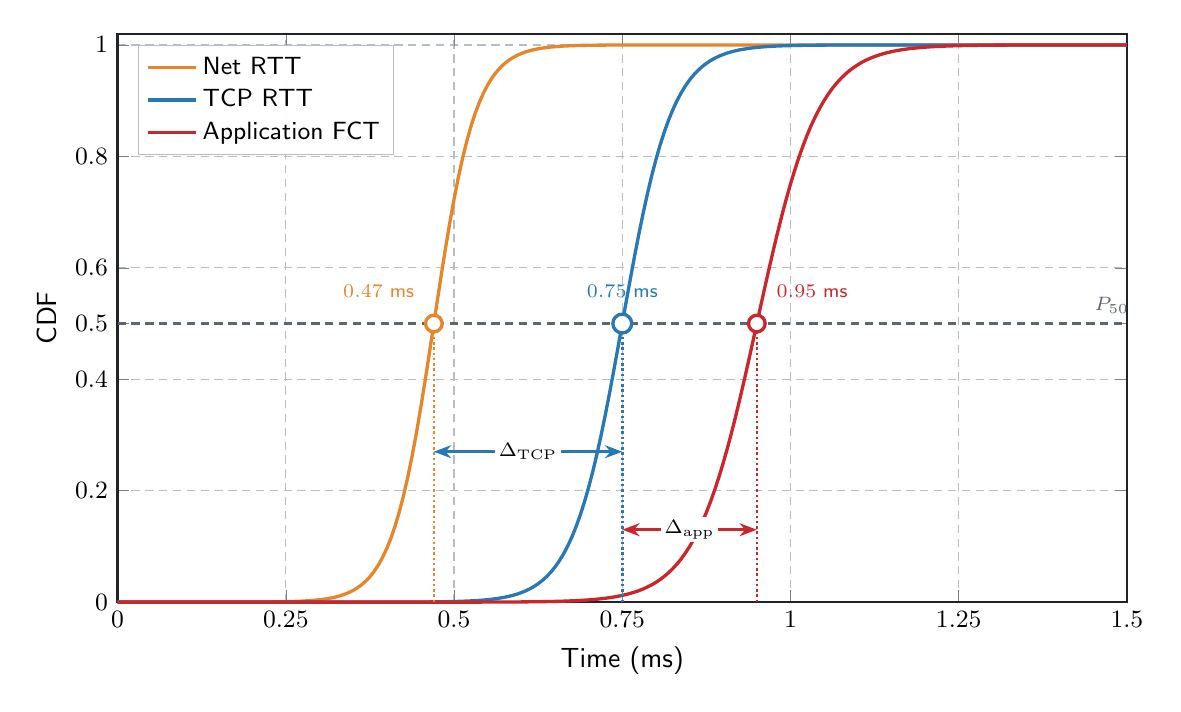
\begin{tikzpicture}[font=\sffamily]
    \begin{axis}[
        width=14.4cm,
        height=8.8cm,
        xmin=0,
        xmax=1.5,
        ymin=0,
        ymax=1.02,
        xlabel={Time (ms)},
        ylabel={CDF},
        axis line style={draw=IorioInk, line width=0.8pt},
        tick label style={font=\sffamily\small},
        label style={font=\sffamily},
        xtick={0,0.25,0.5,0.75,1.0,1.25,1.5},
        ytick={0,0.2,0.4,0.5,0.6,0.8,1.0},
        grid=both,
        major grid style={draw=IorioGrid, densely dashed, line width=0.45pt},
        minor grid style={draw=IorioGrid!60, dotted, line width=0.35pt},
        legend style={
            at={(0.02,0.98)},
            anchor=north west,
            draw=IorioGrid,
            fill=white,
            fill opacity=0.94,
            text opacity=1,
            font=\sffamily\small,
            cells={anchor=west}
        },
        domain=0:1.5,
        samples=241,
        no markers,
        clip=false
    ]
        % P50 anchors: Net RTT 0.47 ms, conceptual TCP RTT 0.75 ms,
        % and reported 1 kB application FCT 0.95 ms.
        \addplot[IorioNet, very thick]
            {1/(1+exp(-32*(x-0.47)))};
        \addlegendentry{Net RTT}

        \addplot[IorioTCP, very thick]
            {1/(1+exp(-27*(x-0.75)))};
        \addlegendentry{TCP RTT}

        \addplot[IorioApp, very thick]
            {1/(1+exp(-22*(x-0.95)))};
        \addlegendentry{Application FCT}

        % Median guide and level-specific P50 markers.
        \draw[draw=IorioMuted, densely dashed, line width=0.8pt]
            (axis cs:0,0.5) -- (axis cs:1.5,0.5)
            node[pos=0.985, above, font=\sffamily\scriptsize, text=IorioMuted]
            {$P_{50}$};

        \draw[draw=IorioNet, densely dotted, line width=0.9pt]
            (axis cs:0.47,0) -- (axis cs:0.47,0.5);
        \draw[draw=IorioTCP, densely dotted, line width=0.9pt]
            (axis cs:0.75,0) -- (axis cs:0.75,0.5);
        \draw[draw=IorioApp, densely dotted, line width=0.9pt]
            (axis cs:0.95,0) -- (axis cs:0.95,0.5);

        \addplot[only marks, mark=square*, mark size=3.0pt,
                 draw=IorioNet, fill=white, very thick, forget plot]
            coordinates {(0.47,0.5)};
        \addplot[only marks, mark=diamond*, mark size=3.4pt,
                 draw=IorioTCP, fill=white, very thick, forget plot]
            coordinates {(0.75,0.5)};
        \addplot[only marks, mark=*, mark size=3.0pt,
                 draw=IorioApp, fill=white, very thick, forget plot]
            coordinates {(0.95,0.5)};

        \node[font=\sffamily\scriptsize, text=IorioNet, anchor=south east]
            at (axis cs:0.455,0.53) {$0.47$ ms};
        \node[font=\sffamily\scriptsize, text=IorioTCP, anchor=south]
            at (axis cs:0.75,0.53) {$0.75$ ms};
        \node[font=\sffamily\scriptsize, text=IorioApp, anchor=south west]
            at (axis cs:0.965,0.53) {$0.95$ ms};

        % Median deltas make the additional cost at each layer explicit.
        \draw[{Stealth[length=2.2mm]}-{Stealth[length=2.2mm]},
              draw=IorioTCP, line width=0.9pt]
            (axis cs:0.47,0.27) --
            node[fill=white, inner sep=1.2pt, font=\sffamily\scriptsize]
            {$\Delta_{\mathrm{TCP}}$}
            (axis cs:0.75,0.27);
        \draw[{Stealth[length=2.2mm]}-{Stealth[length=2.2mm]},
              draw=IorioApp, line width=0.9pt]
            (axis cs:0.75,0.13) --
            node[fill=white, inner sep=1.2pt, font=\sffamily\scriptsize]
            {$\Delta_{\mathrm{app}}$}
            (axis cs:0.95,0.13);
    \end{axis}
\end{tikzpicture}

% Page 2: connection reuse versus repeated TCP/TLS establishment.
% Suggested thesis caption:
% Persistent transport sessions reduce FCT by avoiding repeated connection and
% TLS establishment. This motivates RDG to preserve occurrence-local security
% state and to reuse transport sessions whenever the transaction contract and
% the authorised security policy permit it.
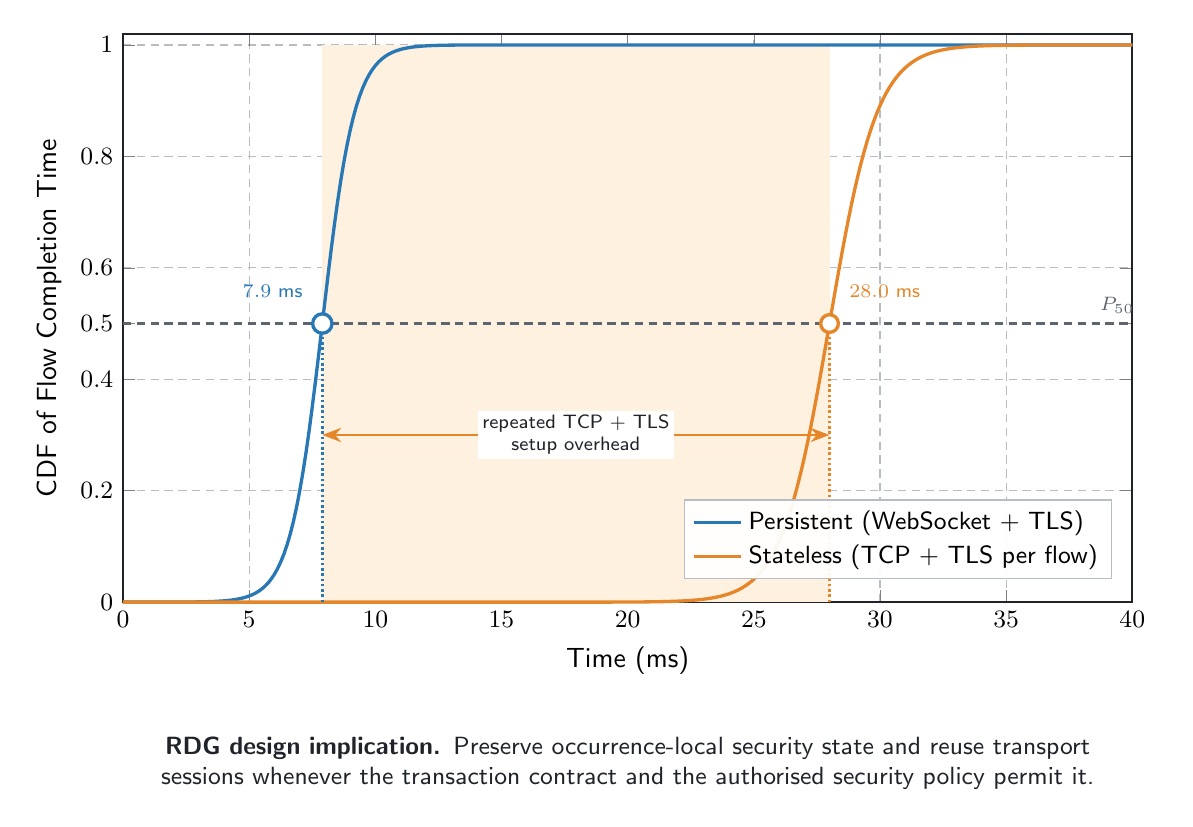
\begin{tikzpicture}[font=\sffamily]
    \begin{axis}[
        width=14.4cm,
        height=8.8cm,
        xmin=0,
        xmax=40,
        ymin=0,
        ymax=1.02,
        xlabel={Time (ms)},
        ylabel={CDF of Flow Completion Time},
        axis line style={draw=IorioInk, line width=0.8pt},
        tick label style={font=\sffamily\small},
        label style={font=\sffamily},
        xtick={0,5,10,15,20,25,30,35,40},
        ytick={0,0.2,0.4,0.5,0.6,0.8,1.0},
        grid=both,
        major grid style={draw=IorioGrid, densely dashed, line width=0.45pt},
        minor grid style={draw=IorioGrid!60, dotted, line width=0.35pt},
        legend style={
            at={(0.98,0.04)},
            anchor=south east,
            draw=IorioGrid,
            fill=white,
            fill opacity=0.94,
            text opacity=1,
            font=\sffamily\small,
            cells={anchor=west}
        },
        domain=0:40,
        samples=321,
        no markers,
        clip=false
    ]
        % The shaded interval represents repeated TCP and TLS setup overhead at P50.
        \path[fill=IorioShade, draw=none]
            (axis cs:7.9,0) rectangle (axis cs:28.0,1);

        \addplot[IorioPersistent, very thick]
            {1/(1+exp(-1.55*(x-7.9)))};
        \addlegendentry{Persistent (WebSocket + TLS)}

        \addplot[IorioStateless, very thick]
            {1/(1+exp(-1.05*(x-28.0)))};
        \addlegendentry{Stateless (TCP + TLS per flow)}

        \draw[draw=IorioMuted, densely dashed, line width=0.8pt]
            (axis cs:0,0.5) -- (axis cs:40,0.5)
            node[pos=0.985, above, font=\sffamily\scriptsize, text=IorioMuted]
            {$P_{50}$};
        \draw[draw=IorioPersistent, densely dotted, line width=0.9pt]
            (axis cs:7.9,0) -- (axis cs:7.9,0.5);
        \draw[draw=IorioStateless, densely dotted, line width=0.9pt]
            (axis cs:28.0,0) -- (axis cs:28.0,0.5);

        \addplot[only marks, mark=diamond*, mark size=3.5pt,
                 draw=IorioPersistent, fill=white, very thick, forget plot]
            coordinates {(7.9,0.5)};
        \addplot[only marks, mark=*, mark size=3.2pt,
                 draw=IorioStateless, fill=white, very thick, forget plot]
            coordinates {(28.0,0.5)};

        \node[font=\sffamily\scriptsize, text=IorioPersistent,
              anchor=south east]
            at (axis cs:7.5,0.53) {$7.9$ ms};
        \node[font=\sffamily\scriptsize, text=IorioStateless,
              anchor=south west]
            at (axis cs:28.4,0.53) {$28.0$ ms};

        \draw[{Stealth[length=2.4mm]}-{Stealth[length=2.4mm]},
              draw=IorioStateless, line width=1.0pt]
            (axis cs:7.9,0.30) --
            node[fill=white, inner sep=1.5pt, align=center,
                 font=\sffamily\scriptsize, text=IorioInk]
            {repeated TCP + TLS\\setup overhead}
            (axis cs:28.0,0.30);

        \node[anchor=north, align=center, text width=13.4cm,
              font=\sffamily\small, text=IorioInk]
            at (axis description cs:0.5,-0.22)
            {\textbf{RDG design implication.} Preserve occurrence-local security
             state and reuse transport sessions whenever the transaction contract
             and the authorised security policy permit it.};
    \end{axis}
\end{tikzpicture}

\end{document}
